\documentclass[a4paper]{article}

\usepackage{times}
\usepackage[ngerman]{babel}
\usepackage[T1]{fontenc}
\usepackage{amsmath}
\usepackage{amsfonts}
\usepackage{graphicx}
\usepackage{chemfig}
\usepackage{mhchem}
\usepackage{fancyhdr}
\usepackage{longtable}
\usepackage{xcolor}
\usepackage{amssymb}

\pagestyle{fancy}
\fancyhf{}
\renewcommand{\headrulewidth}{0,6pt}
\fancyhead[L]{\leftmark}
\fancyhead[R]{\thepage}

\makeatletter
\newcommand*{\rom}[1]{\expandafter\@slowromancap\romannumeral #1@}
\makeatother

\title{\Huge{Organische Chemie\\Lernzettel}}
\date{\today}
\author{\quad\\Baden, Julian\\Hagemann, Florian\\\\Gymnasium Mellendorf\\ABI Jahr 2027}

\begin{document}

\maketitle
\thispagestyle{empty}
\newpage
\tableofcontents \thispagestyle{empty}
\newpage
\pagenumbering{arabic}


%________________________________________________________________________________________________


\section{Stöchiometrie}
Stöchiometrie, auch chemisches Rechnen, ist ein Werkzeug der Chemie, mit welchen man Stoffmengen verhältnisse
nutzen kann, um zum Beispiel Produktmengen oder Volumen zu errechnen.
\subsection{Größen}
\begin{center}
\begin{tabular}{|c|c|c|}
    \hline
    Größe       &Symbol     &Einheit \\\hline
    Atomanzahl  &$N$        &-- \\ 
    Avogrado-Konstante &$N_a$ &$mol^{-1}$ \\
    Stoffmenge &$n$ &$mol$ \\
    Masse &$m$ &$kg$ \\
    Molare Masse &$M$ &$kg \cdot mol^{-1}$ \\
    Volumen &$V$ &$l$ \\
    Molares Volumen &$V_m$ &$l \cdot mol^{-1}$\\ \hline
\end{tabular}
\end{center}

\subsection{Formeln}
\Large
\begin{eqnarray*}
    n &= \dfrac{N}{N_a} \\ [5mm]
    n &= \dfrac{m}{M} \\ [5mm]
    n &= \dfrac{V}{V_m}
\end{eqnarray*}
\normalsize

\subsection{Standartbedinungen und Normbedingungen}
\begin{center}
    \begin{tabular}{|c|c|c|}
        \hline
        Größen &Standartbedingungen &Normbedingungen \\\hline
        Temperatur &$298\;K = 25\;C$ &$273\;K = 0\;C$ \\
        Druck &$1000 \; hPa$ &$1013 \; hPa$ \\
        Molares Volumen &$V_m = 24 \; l \cdot mol^{-1}$ &$V_{mn} = 22,4 \; l \cdot mol^{-1}$ \\\hline
    \end{tabular}
\end{center}



\section{Grundlegendes Wissen}

\subsection{Säuren und Basen nach Brønsted}
Der dänische Chemiker \emph{Brønsted} definierte die \textbf{Brønsted-Säure} als Moleküle oder Ionen, die bei
einer Reaktion Protonen an einen Reaktionspartner abgeben. Deshalb sind diese also \textbf{Protonen-Donatoren}.

\textbf{Brønsted-Basen} sind definiert als Moleküle oder Ionen, welche bei einer Reaktion von einen Reaktionspartner Protonen aufnehmen.
Diese sind daher \textbf{Protonen-Akzeptoren}.

Aus der Definition Brønsteds geht hervor das eine Base imme mit einer Säure zusammen reagiert. Diese Reaktion nennt
man \textbf{Säure-Base-Reaktion}. Ein Beispiel für eine Säure-Base-Reaktion ist die Reaktion zwischen Salzsäure und
Wasser.
\begin{center}
\schemestart
\chemname{\ce{HCl}}{\emph{Säure}} \quad+\quad \chemname{\ce{H_2O}}{\emph{Base}} \arrow{<->} \chemname{\ce{Cl^$\ominus$}}{\emph{Base}} \quad+\quad\chemname{\ce{H_3O^$\oplus$}}{\emph{Säure}}
\schemestop    
\end{center}
Zu erkennen ist das saure Lösungen immer \textbf{Oxonium-Ionen} (\ce{H_3O^$\oplus$}) und Säurerest-Ionen (hier: \ce{Cl^$\ominus$}) enthalten. 

Wasser kann nicht nur als Base mit einer Säure reagieren, sondern auch als Säure mit einer Base. Betrachten wir nun die Reaktion zwischen Wasser und Ammoniak:
\begin{center}
\schemestart
\chemname{\ce{NH_3}}{\emph{Base}} \quad+\quad \chemname{\ce{H_2O}}{\emph{Säure}} \arrow{<->} \chemname{\ce{NH_4^$\oplus$}}{\emph{Säure}} \quad+\quad\chemname{\ce{OH^$\ominus$}}{\emph{Base}}
\schemestop    
\end{center}
Alkalische Lösungen sind von den \textbf{Hydroxid-Ionen}(\ce{OH^$\ominus$}) charakterisiert und enthalten auch Baserest-Ionen (hier: \ce{NH_4^$\oplus$}).
Säuren und Basen reagieren zusammen zu Wasser und den jeweiligen Rest-Ionen.


\subsection{Nucleophile und Elektrophile}
\paragraph{Nucleophile} 
Teilchen sind \textbf{negativ} geladenen Ionen oder Moleküle mit \textbf{Elektronenüberschuss}, zum Beispiel freie Elektronenpaare (Elektronendonatoren).
Sie greifen den Reaktionspartner an Stellen \textbf{niedriger Elektronendichte}, also im Bereich positiver Ladung oder Partialladung an.

Die Stärke eines Nucleophils hängt erstens von seiner \textbf{Ladung} ab, je negativer, desto stärker, und zweitens von seiner
\textbf{Polarisierbarkeit}, welche proportional mit der Größe des Teilchens ist. Das heißt: Je größer das Teilchen, desto besser
kann es polarisiert werden. Ob eine Abgangsgruppe gut oder schlechter ist, ist Analog.

\paragraph{Elektrophile} Teilchen sind Ionen oder Moleküle mit \textbf{Elektronenmangel} beziehungsweise \textbf{Elektronenlücken} (Elektronenakzeptoren).
Sie greifen den Reaktionspartner an Stellen \textbf{hoher Elektronendichte}, also im Bereich negativer Ladung oder Partialladung an.


\subsection{Typische Ionen}
Manche Ionen kommen in der Organik häufig vor. Die Wichtigsten und wie sie heißen ist im folgenden zu finden:
\begin{center}
    \begin{longtable}{c c c}
        Oxoniumion &\ce{H_3O^$\oplus$} &\chemfig{H-\charge{90=\|}{\ce{O}}^{\oplus}(-[:270]H)-H} \\[15mm]
        Hydroxidion &\ce{OH} &\chemfig{H-\charge{0=\|,90=\|,270=\|}{O}^{\;\ominus}}\\ [15mm]
        Primäres Carbokation &-- &\chemfig{R-C^{\oplus}(-[:270]H)-H} \\[15mm]
        Sekundäres Carbokation &-- &\chemfig{R-C^{\oplus}(-[:270]H)-R} \\[15mm]
        Tertiäres Carbokation &-- &\chemfig{R-C^{\oplus}(-[:270]R)-R} 
    \end{longtable}
\end{center}

\subsection{I-Effekt}
Der I-Effekt beschreibt Einflüsse von Atomen und Atomgruppen auf die Elektronendichte und Verteilung in Bindungen.
Er kann sich über mehrere Bindungen auswirken.\\[5mm]
Der \textbf{+I-Effekt erhöht} die $e^-$-Dichte benachtbarter Atome / Atomgruppen. Er wird von z.B. Alkylresten ausgeübt.\\[5mm]
Der \textbf{-I-Effekt verringert} die $e^-$-Dichte benachtbarter Atome / Atomgruppen. Er wird von z.B. F, Cl, O, N und S ausgeübt.\\[5mm]
Schauen wir uns die \textbf{Stabilitätsreihe der Alkylradikale} an:
\begin{center}
    Primäre \quad<\quad Sekundäre \quad<\quad Tertiäre \quad<\quad Methyl\\
\end{center}
Der Grund für diese Anordnung ist der +I-Effekt der Alkylgruppen.

\subsection{Nachweisreaktion}
\begin{center}
    \begin{tabular}{|c | c|} \hline
        \textbf{Nachweisreaktion} & \textbf{Stoff} \\ \hline
        Knallgasprobe &Wasserstoff \\
        Glühspanprobe &Sauerstoff \\
        Kalkwasserprobe &Kohlenstoffdioxid \\
        Entfärbung von Brom &Alken oder Alkin \\
        Beilsteinprobe & Halogenalkan \\ \hline
        Silbernitrat & Weißer Niederschlag: Chlorid \\
        \quad & Weiß-Gelber Niederschlag: Bromid \\
        \quad & Gelber Niederschlag: Iodid \\ \hline
    \end{tabular}
\end{center}



\section{Stoffklassen}
\subsection{Alkane}

Alkane Sind eine Reihe \textbf{Kohlenstoffatome}, mit anliegenden
\textbf{Wasserstoffatomen}. Die Reihe, welche die Alkane bilden, wenn man sie nach der Anzahl C-Atom
ordnet, heißt "homologe Reihe"\\[0,5cm]
\begin{center}
\chemfig{H-C(-[:90]H)(-[:270]H)-C(-[:90]H)(-[:270]H)-H} \hspace{1cm} \textbf{Ethan}\\[0,5cm]
\begin{tabular}{|c|c|c|}
    \hline
    Name        & Molekülformel          & Halbstrukturformel\\ \hline 
    Methan      & \chemfig{C H_4}        & \chemfig{CH_3}\\
    Ethan       & \chemfig{C_2 H_6}      & \chemfig{CH_3 - CH_3}\\
    Propan      & \chemfig{C_3 H_8}      & \chemfig{CH_3 - CH_2 - CH_3}\\
    Butan       & \chemfig{C_4 H_{10}}     & \chemfig{CH_3 - C_2 H_2 - CH_3}\\
    Pentan      & \chemfig{C_5 H_{12}}     & \chemfig{CH_3 - C_3 H_4 - CH_3}\\
    Hexan       & \chemfig{C_6 H_{14}}     & \chemfig{CH_3 - C_4 H_6 - CH_3}\\
    Heptan      & \chemfig{C_7 H_{16}}     & \chemfig{CH_3 - C_5 H_8 - CH_3}\\
    Octan       & \chemfig{C_8 H_{18}}     & \chemfig{CH_3 - C_6 H_{10} - CH_3}\\
    Nonan       & \chemfig{C_9 H_{20}}     & \chemfig{CH_3 - C_7 H_{12} - CH_3}\\
    Decan       & \chemfig{C_{10} H_{22}}  & \chemfig{CH_3 - C_8 H_{14} - CH_3}\\ \hline
\end{tabular}\\[1cm]
\end{center}

Innehalb der Homologen Reihe sind folgende \textbf{Zusammenhänge} zu erkennen:\\
\begin{itemize}
    \item {Viskousität steigt}
    \item {Siede- \& Schmelztemperatur steigt}
    \item {Dichte nimmt zu} \\
\end{itemize}
Diese Zusammenhänge liegen an steigender Intensität von London- / Van-der-Waals-kräfte mit steigender Kettenlänge.\\[0,5cm]

Alkane besitzen folgene \textbf{Eigenschaften}:\\
\begin{itemize}
    \item{keine elektrische Leitfähigkeit}
    \item {sie sind unpolar}\\[1cm]
\end{itemize}


\subsection{Halogenalkane}

Halogenalkane sind Alkane, denen durch \textbf{elektrophile Addition}, aus Alkenen, oder durch
\textbf{radikalische Substitution}, aus Alkanen, ein Halogen addiert wurde. \\

\begin{center}
    \chemfig{H-C(-[:90]H)(-[:270]Br)-C(-[:90]H)(-[:270]H)-H} \hspace{1cm} \textbf{Bromethan}\\[0,5cm]
\end{center}

Halogenalkane sind \textbf{lipophil}, ihre \textbf{Siedetemperatur ist höher als bei Alkanen}.
Bei Mehrfachsubstutution / Mehrfachaddition werden die Halogenalkane \textbf{mit steigender Halogenanzahl reaktionsträger}.\\

Eine Nachweisreaktion für Halogenalkane ist die Beilsteinprobe.



\subsection{Kohlenwasserstoffe mit Mehrfachbindungen}
\subsubsection{Alkene und Alkine}

Alkene sind Kohlenwasserstoffe, welche eine Doppelbindung zwischen zwei C-Atomen besitzen.
Sie wie die Alkane benannt, besitzen aber eine \textbf{-en} Endung. Vor dieser Endung wird die Stelle der Mehrfachbindung geschrieben,
z.B.: Pent-2-en.\\

\begin{center}
    \chemfig{C (-[:240]H)(-[:120]H) = C (-[:60]H)(-[:300]H)} \hspace{1cm} \textbf{Ethen}\\[0,5cm]
\end{center}


Alkine bekommen hingegen die Ändung \textbf{-in}.\\

\begin{center}
    \chemfig{H - C ~ C - H} \hspace{1cm} \textbf{Ethin}\\[0,5cm]
\end{center}


\subsubsection{$\pi$ und $\sigma$ Bindungen}

Elektronenpaare in Mehrfachbindungen haben verschiedene Bindungsstärken. $\pi$-Bindungen (Pi-Bindungen) sind schwächer als $\sigma$-Bindungen (Sigma-Bindungen).
Sie befinden sich sozusagen seitlich von der Mitte der beiden Bindungspartner. Bei Dreifachbindungen gibt es zwei $\pi$-Bindungen.\\
Das heißt bei Reaktionen, bei denen eine Mehrfachbindung gespalten werden, wird immer die $\pi$-Bindung gespalten.



\subsubsection{Mehrfachsubstutution}

Wichtig bei Mehrfachsubstutution und Mehrfachaddition ist die Benennung mit cis- und trans-.\\
\begin{center}
    \chemfig{H-C(-[:90]H)(-[:270]\charge{0=\|,180=\|,270=\_}{Br})=C(-[:90]\charge{0=\|,180=\|,90=---}{Br})(-[:270]H)-H} \hspace{1cm} \textbf{Trans-1,2-dibromethen}\\[0,5cm]
    \chemfig{H-C(-[:90]H)(-[:270]\charge{0=\|,180=\|,270=\_}{Br})=C(-[:90]H)(-[:270]\charge{0=\|,180=\|,270=\_}{Br})-H} \hspace{1cm} \textbf{Cis-1,2-dibromethen}\\[0,5cm]
\end{center}

Eine Nachweisreaktion für Mehrfachbindungen ist die Entfärbung von Bromwasser. Der typische Reaktionsmechanismus der Alkene ist die elektrophile Addition.


\subsection{Alkohole}

Alkohole sind Moleküle mit einer O-H-Gruppe (Hydroxygruppe).\\
Die Alkohole werden auf zwei Weisen unterschieden:
\begin{enumerate}
    \item Wertigkeit:\\
            Die Wertigkeit gibt die Anzahl der OH-Gruppen an. Einwertige haben eine, dreiwertige drei,\dots\\
            Mit mehr OH-Gruppen nimmt die Löslichkeit in Wasser zu, da diese Gruppen polar sind.
    \item Primäre, Sekundäre, Tertiäre\\
            Bei primären Alkoholen ist die OH-Gruppe an ein C-Atom gebunden, welches nur ein anderes anliegende C-Atom hat.
            Bei Sekundären ist sie an ein C-Atom gebunden, an welchem zwei weitere C-Atome gebunden sind.\\
\end{enumerate}


\subsection{Typische Reaktionsmechanismen}
\begin{tabular}{|c|c|} \hline
    Stoffklasse &Typischer Mechanismus \\\hline
    Alkane &Substitution, Eliminierung\\
    Halogenalkan &Nukleophile Substitution, Eliminierung,\\
    Alkene / Alkine &Addition\\
    Alkohole &Oxidation
\end{tabular}



\section{Redoxreaktion}

\subsection{Was ist eine Redoxreaktion}
Eine \textbf{Oxidation} ist definiert als Elektronenabgabe. Der Stoff, der oxidiert wird, ist das \textbf{Reduktionsmittel}.\\\\
Eine \textbf{Reduktion} ist definiert als Elektronenaufnahmen.Der Stoff, der reduziert wird, ist das \textbf{Oxidationsmittel}\\\\
Daraus geht hervor, dass zu einer Oxidation immer eine Reduktion gehört. Eine Redoxreaktion ist also eine Elektronenübertragung.\\\\


\subsection{Oxidationszahlen}
Oxidationszahlen dienen dazu zu bestimmen, welcher Bestandteil einer Redoxreaktion oxidiert und welches reduziert wird.\\\\

\paragraph{Oxidationszahlen werden wie folgt bestimmt:}
\begin{enumerate}
    \item Lewis Formel notieren
    \item Elektronenpaarbindungen werden dem Atom der Bindung mit der höheren Elektronegativität zugeordnet
    \item Oxidationszahl = Anzahl Valenzelektronen - Anzahl aller zugeordneten Elektronen\\\\
\end{enumerate}


\paragraph{Regeln zur Bestimmung der Oxidationszahlen:}
\begin{enumerate}
    \item Atome in elementaren Stoffen haben die Oxidationszahl \textbf{0}
    \item Bei enfachen \textbf{Ionen} entspricht die Oxidationszahl der Ionenladung
    \item \textbf{Fluor} hat in Verbindungen immer die Oxidationszahl \textbf{-\rom{1}}
    \item H hat in Verbindungen immer die Oxidationszahl \textbf{\rom{1}}\\
            Eine Außnahme stellen Hydride dar ($NaH$, $CaH_2$)
    \item Sauerstoff hat in Verbindungen immer die Oxidationszahl \textbf{-\rom{2}}\\
            Eine Außnahme bilden Peroxide und Sauerstofffluoride ($H_2O_2$, $OF_2$)
    \item Die Summe der Oxidationszahlen eines Teilchens entspricht der Gesamtladung des Teilchens.
\end{enumerate}



\section{Reaktionsarten}

\subsection{Reaktionswege der Alkane}
\begin{center}
    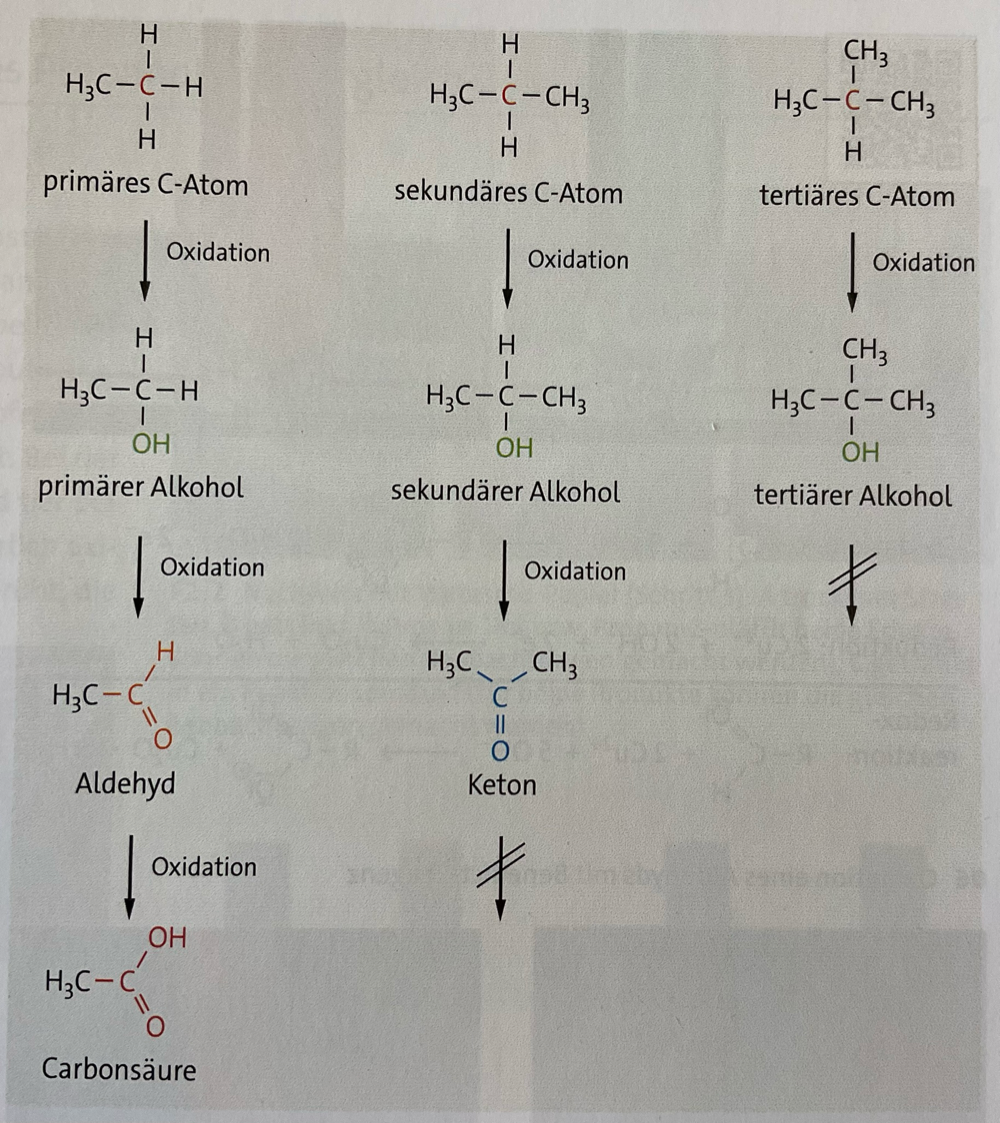
\includegraphics[width=12cm]{Bilder/ReaktionswegeAlkane.png}
\end{center}



\subsection{Radikalische Substitution ($S_R$)}

Bei der Radikalischen Substitution wird ein H-Atom eines Kohlenwasserstoffs durch ein Halogen ersetzt.
Sie läuft in drei Schritten ab:\\

\begin{enumerate}
    \item Ein Halogenmolekül wird homolytisch (=in zwei gleiche Teile) in zwei Radikale, mit jeweils einem freien Elektron \textbf{gespalten}.
         \begin{center}
            \schemestart
                \chemfig{\charge{-180=\|,-90=\|,90=\|}{X} - \charge{0=\|,-90=\|,90=\|}{X}} \quad $\xrightarrow{Energie}$ \quad
                \charge{-180=\|,-90=\|,90=\|,0=\.}{X} \quad + \quad \charge{0=\|,-90=\|,90=\|,-180=\.}{X}
            \schemestop
        \end{center}
    \item Eines dieser Halogenradikale greift ein \textbf{H-Atom} des Kohlenwasserstoffs an und \textbf{spaltet} dieses \textbf{ab}. Es bildet sich ein Halogenwasserstoff und eine Kohlenwasserstoffradikal.
            \begin{center}
                \schemestart
                    \charge{-180=\|,-90=\|,90=\|,0=\.}{X} \quad + \quad \chemfig{H - C (-[90]) (-[-90]) (-[0])} \arrow
                    \chemfig{\charge{-180=\|,-90=\|,90=\|}{X} - H} \quad + \quad \chemfig{\charge{-180=\.}{C} (-[90]) (-[-90])-}
                \schemestop
                \end{center}
    \item Es sind mehrere \textbf{Rekombinationsreaktionen} möglich:
        \begin{enumerate}
            \item Es reagieren ein Halogenradikal und ein Kohlenwasserstoffradikal zu einem Halogenkohlenwasserstoff.\\
                \begin{center}
                \schemestart
                    \charge{-180=\|,-90=\|,90=\|,0=\.}{X} \quad + \quad \chemfig{ \charge{-180=\.}{C} (-[90]) (-[-90]) - } \arrow
                    \chemfig{ \charge{-180=\|,-90=\|,90=\|}{X} - C (-[90]) (-[-90]) - }
                \schemestop
                \end{center}
            \item Es reagieren zwei Kohlenwasserstoffradikale miteinander, wobei ein einzelnes Kohlenwasserstoffmolekül aus der Summe beider entsteht.
                \begin{center}
                \schemestart
                    \chemfig{\phantom{R}-\charge{0=\.}{C} (-[90]) (-[-90])} \quad + \quad \chemfig{ \charge{-180=\.}{C} (-[90]) (-[-90]) - } \arrow
                    \chemfig{\phantom{R}-C (-[90]) (-[-90]) - C (-[90]) (-[-90])-}
                \schemestop
                \end{center}
            \item Es reagieren zwei freien Halogenradikale miteinander, wobei ein Halogenmolekül entsteht und ein Kohlenwasserstoffradikal zurückbleibt.
                \begin{center}
                \schemestart
                    \charge{-180=\|,-90=\|,90=\|,0=\.}{X} \quad + \quad \charge{0=\|,-90=\|,90=\|,-180=\.}{X} \arrow
                    \chemfig{\charge{-180=\|,-90=\|,90=\|}{X} - \charge{0=\|,-90=\|,90=\|}{X}}
                \schemestop
                \end{center}
        \end{enumerate}
\end{enumerate}



\subsection{Nucleophile Substitution}

Bei der Nucleophilen Substitution wird ein Halogen eines Halogenkohlenwasserstoffs durch ein Nucleophil ersetzt.\\
Es gibt zwei verschiedene Arten nucleophiler Substitution. Die \textbf{monomolekulare $S_N1$} und die \textbf{bimolekulare $S_N2$}.\\
Bei der $S_N1$ wir zuerst das Halogen abgespalten und ein \ce{X^-}-Ion und ein Kohlenwasserstoffradikal entstehen.
Danach reagiert erst das Nucleophil mit diesem Radikal.\\\\
Bei der $S_N2$ passieren diese zwei Schritte gleichzeitig. Es sind also zeitweise sowohl Halogen, als auch Nucleophil an das selbe C-Atom des Kohlenwasserstoffs gebunden.\\

\subsubsection{$S_N1$}

\begin{enumerate}
    \item Schritt\\
        \begin{center}
        \schemestart
            \chemfig{\phantom{Q}- C (-[90]) (-[-90]) - \charge{0=\|,-90=\|,90=\|}{X}} \arrow
            \chemfig{\phantom{Q}- \ce{C^+} (-[90]) (-[-90])} \quad + \quad \chemfig{\charge{0=\|,-90=\|,90=\|,-180=\|}{\ce{X}}^{\;\ominus}}
        \schemestop
        \end{center}
    \item Schritt\\
        \begin{center}
        \schemestart
            \chemfig{\phantom{Q}- \ce{C^+} (-[90]) (-[-90])} \quad + \quad \chemfig{\charge{90=\|,-90=\|,-180=\|}{\ce{O}}^{\;\ominus} - H} \arrow
            \chemfig{\phantom{Q}- C (-[90]) (-[-90]) - \charge{90=\|,-90=\|}{O} - H}
        \schemestop
        \end{center}
\end{enumerate}

Bei der $S_N1$ bestimmt der erste Schritt die Geschwindigkeit.\\\\

\subsubsection{$S_N2$}

\begin{center}
    \schemestart
        \chemfig{H-\charge{90=\|,-90=\|,0=\|}{\ce{O}}^{\;\ominus}} \quad + \quad \chemfig{\phantom{Q}- C (-[90]) (-[-90]) - \charge{0=\|,-90=\|,90=\|}{X}} \arrow
        \chemfig{H - \charge{90=\|,-90=\|}{\ce{O}}^{\;\delta-} -[,,,,dash pattern=on 3pt off 3pt] C (-[1]) (-[3]) (-[-90]) -[,,,,dash pattern=on 3pt off 3pt] \charge{0=\|,-90=\|,90=\|}{\ce{X}}^{\;\delta-}} \arrow
    \schemestop
    \\[0,5cm]
    \schemestart
        \chemfig{H - \charge{90=\|,-90=\|}{O} - C (-[0]) (-[1]) (-[7])} \quad + \quad \chemfig{\charge{90=\|,-90=\|,0=\|,-180=\|}{\ce{X}}^{\;\ominus}}
    \schemestop
\end{center}

\subsubsection{Vergleich}
Nach welchen Mechanismus die $S_N$ abläuft, ist von der Struktur des Halogenalkans und dem EInfluss des
Nucleophils abhängig. \\
\begin{center}
\begin{tabular}{c | p{27.5mm} | p{27.5mm} | p{27.5mm} |}
    \quad &Anzahl der an der Reaktion beteiligten Teilchen &Abspaltung der Abgangsgruppe und Anlagerung des Nucleophils &Bindungsverhältnis im Halogenalkan \\ \hline
    $S_N1$ &$1 \implies$ monomolekular &nacheinander in zwei Schritten &tertiäres C-Atom \\ \hline
    $S_N2$ &$2 \implies$ bimolekular &gleichzeitig in einem Schritt &primäres C-Atom
\end{tabular}
\end{center}

\subsection{Elektrophile Addition}
Bei einer elektrophile Addition lagern sich Elektrophile an die Doppelbindungen ungesättigter Moleküle.
Diese ist bimolekular und Zweischrittig.

\begin{enumerate}
    \item Schritt\\
        Man starte mit folgenden Edukten:\\ 
        \begin{center}
        \schemestart
            \chemfig{C (-[:240])(-[:120]) = C (-[:60])(-[:300])} \quad + \quad \chemfig{\charge{90=\|,-90=\|,-180=\|}{\ce{X}}-\charge{90=\|,-90=\|,0=\|}{\ce{X}}}
        \schemestop \\ [5mm]
        \end{center}
        Das Halogenmolekül wird von der Doppelbindung \emph{polarisiert}: Es bildet sich der $\pi$-Komplex. \\ 
        \begin{center}
        \schemestart
            \chemfig{C (-[:240])(-[:120]) = C (-[:60])(-[:300])} \quad + \quad \chemfig{\charge{90=\|,-90=\|,-180=\|}{\ce{X}}^{\delta -}-\charge{90=\|,-90=\|,0=\|}{\ce{X}}^{\; \delta +}}
        \schemestop \\ [5mm]
        \end{center}
        Durch die heterolytische Spaltung des Halogenmoleküls bildet sich der $\sigma$-Komplex. \\
        \begin{center}
        \schemestart
            \chemfig{[:-30]C(-[:240])(-[:120])*3(-\quad\charge{0=\|,-90=\|,-180=\|}{\ce{X}}^{\;\oplus}-C (-[:60])(-[:300])-)} \quad+\quad \chemfig{\charge{0=\|,90=\|,180=\|,270=\|}{\ce{X}}^{\;\ominus}}
        \schemestop \\ [5mm]
        \end{center}
    \newpage\item Schritt\\
        Nun greift das Halogenid von der Rückseite an. Es ensteht folgendes Produkt:\\
        \begin{center}
        \schemestart
            \chemfig{-C ([:90]-\charge{0=\|,90=\|,180=\|}{\ce{X}})  ([:270]-) - C ([:270]-\charge{0=\|,270=\|,180=\|}{\ce{X}})  ([:90]-) -}
        \schemestop 
        \end{center}
\end{enumerate}


\subsection{Eleminierungsreaktion}
Bei der Eleminierungsreaktion werden zwei Atome oder Atomgruppen von benachbarten C-Atomen abgespalten ohne, dass diese durch irgentwas ersetzt werden.
Dadurch entsteht zwischen den beiden C-Atomen eine Mehrfachbindung.\\
In folgenden Beispielen werden von einem Halogenalkan mit Hilfe eines Hydroxid-Ions ein Halogen- und ein H-Atom abgespalten.\\

\subsubsection{$E1$}
Die $E1$ Reaktion verläuft, wie auch die $S_N1$ Reaktion, monomolekular in zwei Schritten.\\
\begin{enumerate}
    \item Schritt\\
        Ein Halogen wird abgespalten.
        \begin{center}
        \schemestart
            \chemfig{H-C(-[90])(-[-90])-C(-[90]\charge{90=\|,-180=\|,0=\|}{Br})(-[-90])-C(-[90])(-[-90])(-[0])}
        \schemestop \\ [5mm]
        \end{center}
        Es entsteht ein Carbeniumion, welches vom +I-Effekt der benachbarten C-Atome stabilisiert wird, und ein Halogenid.
        \begin{center}
            \schemestart
                \chemfig{H-C(-[90])(-[-90])-C^{\;\oplus}(-[-90])-C(-[90])(-[-90])(-[0])} \quad+\quad \chemfig{\charge{0=\|,90=\|,-90=\|,-180=\|}{Br}^{\;\ominus}}
            \schemestop \\ [5mm]
        \end{center}
    \newpage\item Schritt\\
        Das Nukleophil (Hydroxid-Ion) greift ein H-Atom an und spaltet dieses ab. Das Elektronenpaar zwischen H- und C-Atom bildet eine Doppelbindung
        zwischen diesem C-Atom und dem, von welchem das Halogen abgespalten wurde. Das entstehende Kohlenwasserstoff ist ein Alken.
        \begin{center}
            \schemestart
                \chemfig{C(-[3])(-[5]) = C(-[-90]) - C(-[90])(-[-90])(-[0])} \quad+\quad \chemfig{\charge{45=\|,135=\|}{O}(-[5]H)(-[7]H)}
            \schemestop \\ [5mm]
        \end{center}
\end{enumerate}


\subsubsection{$E2$}
Die $E2$ Reaktion verläuft, wie die $SN_2$ Reaktion, bimolekular in einem Schritt.\\


Ein Nukleophil greift ein Proton an und spaltet dieses ab.
\begin{center}
\schemestart
    \chemfig{H - \charge{0=\|,90=\|,-90=\|}{O}^{\;\ominus}} \quad+\quad \chemfig{H-C(-[90])(-[-90]) - C(-[-90])(-[90] \charge{90=\|,0=\|,180=\|}{Br})-C(-[90])(-[-90])(-[0])}
\schemestop \\ [5mm]
\end{center}

Dadurch bildet das zurückgebliebene Elektronenpaar eine C=C-Doppelbindung und das Halogen des anderen C-Atoms wird abgespalten.
\begin{center}
\schemestart
    \chemfig{\charge{45=\|,135=\|}{O}(-[5]H)(-[7]H)} \quad+\quad \chemfig{C(-[3])(-[5]) = C(-[-90]) - C(-[90])(-[-90])(-[0])} \quad+\quad \chemfig{\charge{0=\|,90=\|,-180=\|,-90=\|}{Br}^{\;\ominus}}
\schemestop \\ [5mm]
\end{center}

Die $E2$ Reaktion wird bei einer starken Base favorisiert, während die $E1$ eher bei schwachen Basen stattfindet.



\subsubsection{Saytzeff Regel}
Die Saytzeff Regel ermöglicht eine Vorhersage über das bei einer chemischen Eliminierungsreaktion entstehende Produkt.
Sie besagt, dass bei einer E-Reaktion mehr Produkt von von dem Kohlenwasserstoff mit der thermodynamisch günstigeren Doppelbindung entsteht.
Das heißt, dass häufiger vom wasserstoffärmeren Atom ein Proton abgespalten wird.\\[5mm]
\chemfig{C(-[-180]H)(-[90]H)(-[-90]H)-C(-[90]H)=C(-[-90]H)-C(-[90]H)(-[-90]H)-H} \\[5mm]
ist somit häufiger Produkt einer Eliminierung von Butan als\\[5mm]
\chemfig{C(-[3]H)(-[5]H)=C(-[90]H)-C(-[90]H)(-[-90])-C(-[0]H)(-[90]H)(-[-90])-H}\\[5mm]


\subsubsection{Dehydratisierung}
Die Dehydratisierung ist eine Unterart der Eleminierungsreaktion $E1$. Die Dehydratisierung ist die Abspaltung von Wasser in Folge einer
Reaktion. Sie ist eine typische Reaktion von Alkoholen. Die Dehydratisierung verläuft in drei Schritten ab.\\
Im folgenden Beispiel wird Alkohol mithilfe des katalyastors $H_3O$(Ein Oxoniumion) zu Propen und und Wasser.\\\\

\begin{center}
\schemestart
    \chemfig{\phantom{Q}-C(-[90])(-[-90])-C(-[90])(-[-90]\charge{0=\|,-180=\|}{O}(-[-90]H))-C(-[90])(-[-90])-} \quad+\quad \chemfig{H-\charge{90=\|}{O}^{\;\oplus}(-[-90]H)-H}
\schemestop \\[5mm]
\end{center}

\begin{enumerate}
    \item Schritt\\
        Das Oxoniumion gibt ein ein Proton ($H^{\oplus}$) an den Sauerstoff der OH-Gruppe ab.\\
        \begin{center}
        \schemestart
            \chemfig{\phantom{Q}-C(-[90])(-[-90])-C(-[90])(-[-90]\charge{-180=\|}{O}^{\oplus}(-[45]H)(-[135]H))-C(-[90])(-[-90])-} \quad+\quad \chemfig{\charge{45=\|,135=\|}{O}(-[45]H)(-[135]H)}
        \schemestop \\[5mm]
        \end{center}
    \item Schritt\\
        Das entstandene Alkoxoniumion spaltet ein Wassermolekül ab, da dieses eine stark positive Ladung besitzt.
        Es entsteht ein Carboxoniumion. Das C-Atom, von dem das $H_2O$ abgespalten wurde, heißt $\alpha$\\
        \begin{center}
        \schemestart
            \chemfig{\phantom{Q}-C(-[90])(-[-90])-C^{\oplus}(-[90])-C(-[90])(-[-90])-} \quad+\quad \chemfig{\charge{45=\|,135=\|}{O}(-[45]H)(-[135]H)}
        \schemestop \\[5mm]
        \end{center}
    \item Schritt\\
        Durch ein Wassermolekül wird ein Proton von einem benachbarten C-Atom des C-Atoms, von dem das $H_2O$ abgespalten wurde, abgespalten.
        Dieses C-Atom heißt $\beta$ Der katalyastors ($H_3O$) wird erneuert und es entsteht ein Alken.\\
        \begin{center}
        \schemestart
            \chemfig{\phantom{Q}-C(-[90])(-[-90])-C(-[90])=C(-[1])(-[7])} \quad+\quad \chemfig{H-\charge{90=\|}{C}^{\oplus}(-[-90]H)-H}
        \schemestop \\[5mm]
        \end{center}
\end{enumerate}



\subsection{Oxidation von Alkoholen}

\subsubsection{Oxidation primärer Alkohole}
\begin{center}
\schemestart
\chemfig{H-C(-[90]H)(-[-90]H)-C^{\color{red}-\rom{1}\color{black}}(-[90]H)(-[-90]H)-\charge{90=\|,-90=\|}{O}-H} \quad+\quad \chemfig{Cu^{\color{red}\rom{2}\color{black}}=\charge{45=\|,-45=\|}{O}} \arrow
\schemestop \\[5mm]
\schemestart
\chemfig{H-C(-[90]H)(-[-90]H)-C^{\color{red}\rom{1}\color{black}}(-[-135]\charge{90=\|,0=\|}{O})(-[135]H)} \quad+\quad \chemfig{Cu^{\color{red}0\color{black}}} \quad+\quad \chemfig{\charge{135=\|,45=\|}{O}(-[5]H)(-[7]H)}
\schemestop \\[5mm]
\end{center}

Das Kupfer nimmt zwei Elektronen auf und wird reduziert.\\
Das C-Atom gibt zwei Elektronen ab und wird oxidiert.\\
\begin{center}
    $\Rightarrow$ \textbf{Primäre Alkohole $\xrightarrow{Redoxreaktion}$ Aldehyde}
\end{center}

\subsubsection{Oxidation sekundärer Alkohole}
\begin{center}
\schemestart
\chemfig{H-C(-[90]H)(-[-90]H)-C^{\color{red}0\color{black}}(-[90]H)(-[-90]\charge{0=\|,-180=\|}{O}(-[-90]H))-C(-[90]H)(-[-90]H)-H} \quad+\quad \chemfig{Cu^{\color{red}\rom{2}\color{black}}=\charge{45=\|,-45=\|}{O}} \arrow
\schemestop \\[5mm]
\schemestart
\chemfig{H-C(-[90]H)(-[-90]H)-C^{\color{red}\rom{2}\color{black}}(=[-90]\charge{-135=\|,-45=\|}{O})-C(-[90]H)(-[-90]H)-H} \quad+\quad \chemfig{Cu^{\color{red}0\color{black}}} \quad+\quad \chemfig{\charge{135=\|,45=\|}{O}(-[5]H)(-[7]H)}
\schemestop \\[5mm]
\end{center}

\begin{center}
    $\Rightarrow$ \textbf{Sekundärer Alkohole $\xrightarrow{Redoxreaktion}$ Ketone}
\end{center}

\subsubsection{Oxidation tertiärer Alkohole}
\begin{center}
\schemestart
\chemfig{H-C(-[90]H)(-[-90]H)-C^{\color{red}0\color{black}}(-[90]C(-[90]H)(-[0]H)(-[-180]H))(-[-90]\charge{0=\|,-180=\|}{O}(-[-90]H))-C(-[90]H)(-[-90]H)-H} \quad+\quad \chemfig{Cu^{\color{red}\rom{2}\color{black}}=\charge{45=\|,-45=\|}{O}} \qquad \Large $\nrightarrow$ \normalsize
\schemestop \\[5mm]
\end{center}

Tertiäre Alkohol können nicht oxidiert werden.

\begin{center}
    $\Rightarrow$ \textbf{Tertiäre Alkohole $\nRightarrow$}
\end{center}


\end{document}